\documentclass[conference]{IEEEtran}
\usepackage[utf8]{inputenc}
\usepackage[T1]{fontenc}
\usepackage{cite}
\usepackage{amsmath,amssymb,amsfonts}
\usepackage{algorithm,algorithmic}
\usepackage{float}
\makeatletter
\renewcommand{\ALG@name}{Algoritmo}
\renewcommand{\thealgorithm}{\arabic{algorithm}:}
\makeatother
\usepackage{graphicx}
\usepackage{textcomp}

\usepackage[table]{xcolor}
\usepackage{tabularx}
\usepackage{url, hyperref}
\usepackage{booktabs}
\usepackage{array}
\usepackage{listings}

\renewcommand{\figurename}{Figura}
\renewcommand{\tablename}{Tabela}
\renewcommand{\refname}{Referências}

% Ajuste para evitar esticamento vertical de parágrafos e lacunas (espaçamentos indesejados)
\raggedbottom

\definecolor{azul}{HTML}{1F4E79}
\definecolor{fundotab}{HTML}{F2F2F2}

\def\BibTeX{{\rm B\kern-.05em{\sc i\kern-.025em b}\kern-.08em
    T\kern-.1667em\lower.7ex\hbox{E}\kern-.125emX}}

\title{Trabalho Prático Individual I: Estruturas em Árvores Avançadas\\
{\large Modelagem, Implementação e Análise Comparativa de Estruturas em Árvore Especializadas}}

\author{\IEEEauthorblockN{Gabriel Alves Faria}
\IEEEauthorblockA{\textit{Graduando em Engenharia de Computação} \\
\textit{Centro Federal de Educação Tecnológica de Minas Gerais (CEFET-MG -- Campus V)}\\
Divinópolis, Brasil \\
gabrielalvesfaria@gmail.com}
}

\begin{document}

\maketitle

\begin{abstract}
Este trabalho apresenta o estudo, implementação em C++17 e análise comparativa de cinco estruturas de dados em árvore especializadas: Trie, Árvore Patricia (Radix Tree compacta), Árvore Splay, Árvore Treap e KD-Tree. Tais estruturas abordam limitações das árvores binárias de busca (BST) e AVL em cenários como indexação por prefixos, localidade de acesso, balanceamento probabilístico e particionamento espacial multidimensional. O trabalho integra fundamentação teórica, rastreamento visual das transformações estruturais, análise formal de complexidade assintótica e avaliação experimental de desempenho em diferentes padrões e tamanhos de dados ($N$ até $100.000$). Os resultados práticos confirmaram a convergência com as estimativas teóricas, evidenciando o impacto de constantes ocultas e decisões de projeto no desempenho observado.
\end{abstract}

\begin{IEEEkeywords}
Estruturas de Dados, Árvores Avançadas, Trie, Árvore Patricia, Árvore Splay, Árvore Treap, KD-Tree, Análise de Complexidade.
\end{IEEEkeywords}

% =====================================================================
\section{Introdução e Fundamentação Teórica}

As árvores binárias de busca (BST) e suas variantes balanceadas, como a árvore AVL, constituem estruturas fundamentais para a organização e recuperação eficiente de dados ordenados. Entretanto, tais estruturas apresentam limitações em contextos específicos, como a representação de conjuntos de strings com prefixos compartilhados, a adaptação dinâmica a padrões de acesso desiguais, o balanceamento probabilístico com baixo custo de implementação e a organização de dados multidimensionais. Nesse contexto, estruturas especializadas -- Trie, Árvore Patricia, Árvore Splay, Árvore Treap e KD-Tree -- foram concebidas para atender a demandas particulares, cada uma explorando estratégias distintas de organização, balanceamento e indexação. Este trabalho estuda, implementa e compara essas cinco estruturas, relacionando seus fundamentos teóricos ao comportamento observado experimentalmente.

\subsection{Trie (Árvore de Prefixos)}

A Trie, proposta originalmente por Fredkin~\cite{fredkin1960}, é uma estrutura hierárquica destinada à representação eficiente de conjuntos de strings. Diferentemente das árvores de busca convencionais, cada nó da Trie não armazena uma chave completa, mas sim um símbolo do alfabeto utilizado, de modo que o caminho percorrido da raiz até um nó marcado como terminal corresponde a uma chave armazenada na estrutura. Essa organização permite que chaves com prefixos comuns compartilhem os mesmos nós iniciais, reduzindo a redundância de armazenamento em conjuntos de dados com alta sobreposição de prefixos.

A complexidade das operações fundamentais -- inserção, busca e remoção -- é da ordem de $O(m)$, em que $m$ representa o comprimento da chave manipulada, sendo independente do número total de chaves armazenadas na estrutura. Essa característica torna a Trie particularmente adequada para aplicações como sistemas de autocompletar, corretores ortográficos, dicionários e processamento de linguagem natural. Como limitação, observa-se um consumo elevado de memória quando o alfabeto utilizado é extenso e os prefixos compartilhados entre as chaves são escassos, uma vez que cada símbolo distinto corresponde a um nó individual.

\subsection{Árvore Patricia (Radix Tree Compacta)}

A árvore Patricia, introduzida por Morrison~\cite{morrison1968}, constitui uma variação compacta da Trie, concebida para eliminar a ineficiência decorrente de nós com um único filho. Nessa estrutura, sequências de nós unários são colapsadas em uma única aresta, rotulada por uma subcadeia de caracteres, de modo que cada nó interno passa a possuir, necessariamente, pelo menos dois filhos. Essa compactação assegura que o número de nós internos da estrutura seja proporcional ao número de chaves armazenadas, e não ao comprimento total dessas chaves, resultando em economia significativa de espaço em relação à Trie tradicional.

As operações de busca, inserção e remoção mantêm complexidade $O(m)$, sendo $m$ o comprimento da chave buscada. A árvore Patricia é amplamente empregada em tabelas de roteamento IP, nas quais se realiza a busca pelo prefixo mais longo correspondente (\textit{longest prefix match}), bem como em índices compactos para conjuntos esparsos de strings e em variantes como a Merkle Patricia Trie, empregada no armazenamento de estado em sistemas blockchain.

\subsection{Árvore Splay}

A árvore Splay, apresentada por Sleator e Tarjan~\cite{sleator1985}, é uma árvore binária de busca autoajustável, caracterizada pela reorganização dinâmica de sua estrutura a cada operação de acesso. Após uma busca, inserção ou remoção, o nó acessado é deslocado até a raiz por meio de uma sequência de rotações -- denominada \textit{splaying} --, que contempla três casos fundamentais: \textit{zig}, \textit{zig-zig} e \textit{zig-zag}, conforme a posição relativa do nó em relação a seu genitor e avô.

Diferentemente da árvore AVL, a Splay não mantém um fator de balanceamento explícito; o equilíbrio da estrutura resulta, de forma amortizada, das sucessivas reorganizações provocadas pelos acessos. Essa propriedade confere à árvore Splay uma característica de localidade temporal, na qual elementos acessados recentemente permanecem próximos da raiz, favorecendo sequências de acesso com padrões desiguais. A análise amortizada, fundamentada no método do potencial, demonstra que o custo por operação é $O(\log n)$, ainda que uma operação isolada possa, no pior caso, custar $O(n)$. Essa estrutura encontra aplicação em sistemas de cache e em outras estruturas de dados avançadas, como as \textit{link-cut trees}.

\subsection{Árvore Treap (Tree + Heap)}

A árvore Treap combina as propriedades de uma árvore binária de busca com as de um heap, associando a cada nó, simultaneamente, uma chave e uma prioridade atribuída de forma aleatória. Enquanto as chaves respeitam a propriedade de ordenação característica das BSTs, as prioridades obedecem à propriedade de heap, o que garante, com alta probabilidade, uma estrutura balanceada. O fundamento conceitual da Treap remonta à noção de árvore cartesiana, descrita por Vuillemin~\cite{vuillemin1980}, tendo sido formalizada e analisada probabilisticamente por Seidel e Aragon~\cite{seidel1996}.

Para um conjunto fixo de chaves, a configuração da árvore é unicamente determinada pelas prioridades atribuídas, e rotações são empregadas para restaurar a propriedade de heap sempre que uma inserção ou remoção viola essa condição. As operações fundamentais apresentam complexidade esperada $O(\log n)$, decorrente diretamente da aleatoriedade das prioridades, o que confere à Treap um balanceamento probabilístico obtido com relativa simplicidade de implementação, em contraste com os mecanismos determinísticos da árvore AVL.

\subsection{KD-Tree (k-dimensional Tree)}

A KD-Tree, proposta por Bentley~\cite{bentley1975}, é uma estrutura espacial destinada à organização de pontos em espaços multidimensionais. Cada nível da árvore realiza o particionamento do espaço segundo uma dimensão distinta -- de forma cíclica entre as $k$ dimensões --, dividindo o conjunto de pontos por meio de um hiperplano perpendicular ao eixo escolhido.

A construção da estrutura apresenta complexidade $O(n \log n)$, enquanto a busca pelo vizinho mais próximo (\textit{nearest neighbor search}) alcança, em média, complexidade $O(\log n)$, podendo degradar-se para $O(n)$ em espaços de alta dimensionalidade, fenômeno conhecido como maldição da dimensionalidade. Operações de inserção e remoção, por sua vez, tendem a desbalancear a estrutura ao longo do tempo, exigindo, em alguns casos, reconstruções periódicas. A KD-Tree é amplamente utilizada em sistemas de informação geográfica (GIS), processamento de imagens, algoritmos de aprendizado de máquina baseados em vizinhança ($k$-NN), computação gráfica e robótica.

\subsection{Diferenças em relação a BST e AVL}

As cinco estruturas estudadas divergem da BST/AVL em pelo menos um de três eixos: (i) a chave manipulada é uma string decomposta em símbolos (Trie, Patricia), e não um valor atômico comparável diretamente; (ii) o balanceamento é obtido por um mecanismo alternativo ao fator de balanceamento explícito da AVL -- reorganização amortizada por acesso (Splay) ou aleatoriedade de prioridades (Treap); ou (iii) a chave é multidimensional, exigindo alternância do critério de comparação por nível (KD-Tree). A AVL garante $O(\log n)$ no pior caso à custa de rotações determinísticas a cada desbalanceamento; Splay e Treap trocam essa garantia estrita por simplicidade de implementação, aceitando complexidade amortizada ou esperada, respectivamente.

% =====================================================================
\section{Projeto e Implementação das Estruturas}

As cinco estruturas foram implementadas em C++17, cada uma em um arquivo próprio (\texttt{Splay.cpp}, \texttt{Treap.cpp}, \texttt{AvoreTrie.cpp}, \texttt{patricia.cpp}, \texttt{KDTree.cpp}), compartilhando um módulo comum (\texttt{Arvores.h} / \texttt{Padronizar.cpp}) responsável pela leitura e normalização dos arquivos de entrada e pela gravação das medições de tempo em CSV. Todas seguem o mesmo padrão de execução: leem um arquivo de dados, executam operações em lote medindo o tempo com \texttt{std::chrono}, e exportam uma demonstração pequena em formato Graphviz (\texttt{.dot}) para inspeção visual.

\subsection{Árvore Patricia}
Cada nó armazena um mapa de filhos indexado pelo primeiro caractere do rótulo da aresta (\texttt{std::map<char, NoPatricia*>}), e cada aresta carrega uma subcadeia (\texttt{std::string}) em vez de um único símbolo. A inserção calcula o maior prefixo comum entre a chave e o rótulo de uma aresta existente; quando esse prefixo é parcial, a aresta é dividida em dois nós, um dos quais passa a ter exatamente dois filhos, preservando o invariante de compactação. A remoção localiza o nó terminal, desmarca-o e, quando o nó resultante passa a ter um único filho e não é mais terminal, funde a aresta remanescente com a de seu filho único, restaurando a compactação. O Algoritmo~\ref{alg:patricia} descreve a divisão de nós (\textit{split}) realizada durante a inserção.

\begin{algorithm}[H]
\caption{Divisão de Nós (Split) e Fusão (Merge) na Patricia Trie}
\label{alg:patricia}
\begin{algorithmic}[1]
\REQUIRE Nó atual $N$, palavra restante $P$
\STATE $idx \gets P[0] - \text{'a'}$
\STATE $filho \gets N.filho[idx]$
\IF{$filho = \text{NULL}$}
    \STATE $N.filho[idx] \gets
    \text{novo Nó}(P, \text{isWord}=\text{true})$
    \RETURN
\ENDIF
\STATE $k \gets
\text{calcularPrefixoComum}(P, filho.rotulo)$
\IF{$k < |filho.rotulo|$}
    \STATE $prefixo \gets filho.rotulo[0 \dots k-1]$
    \STATE $fimRotulo \gets
    filho.rotulo[k \dots |filho.rotulo|-1]$
    \STATE $meio \gets
    \text{novo Nó}(prefixo, \text{isWord}=\text{false})$
    \STATE $filho.rotulo \gets fimRotulo$
    \STATE $meio.filho[fimRotulo[0]-\text{'a'}]
    \gets filho$
    \IF{$k = |P|$}
        \STATE $meio.isWord \gets \text{true}$
    \ELSE
        \STATE $meio.filho[P[k]-\text{'a'}]
        \gets \text{novo Nó}(P[k \dots |P|-1], \text{true})$
    \ENDIF
    \STATE $N.filho[idx] \gets meio$
\ENDIF
\end{algorithmic}
\end{algorithm}

\subsection{Árvore Trie}
Cada nó mantém um vetor fixo de 26 ponteiros (\texttt{NoTrie* filhos[26]}), um por letra do alfabeto (as palavras de entrada são normalizadas -- minúsculas, sem acentuação -- antes da inserção), e uma marcação booleana de fim de palavra. A inserção percorre a palavra caractere a caractere, criando nós ausentes; a busca por prefixo reaproveita o mesmo percurso, retornando verdadeiro assim que todos os caracteres do prefixo são consumidos, independentemente da marcação de fim de palavra do nó final. A remoção desmarca o nó terminal e libera nós que ficam sem filhos e sem marcação, subindo pela árvore até encontrar um nó ainda necessário. O Algoritmo~\ref{alg:trie} resume a inserção e a busca exata.

\begin{algorithm}[H]
\caption{Inserção e Busca na Árvore Trie}
\label{alg:trie}
\begin{algorithmic}[1]
\REQUIRE Nó raiz $R$, palavra $W$
\STATE \textbf{procedimento} $\text{Inserir}(R, W)$
\STATE \quad $curr \gets R$
\STATE \quad \textbf{para cada} $c \in W$ \textbf{faça}
\STATE \quad \quad $idx \gets \text{tolower}(c) - \text{'a'}$
\STATE \quad \quad \textbf{se} $curr.children[idx] = \text{NULL}$ \textbf{então}
\STATE \quad \quad \quad $curr.children[idx] \gets \text{novo Nó Trie}()$
\STATE \quad \quad \textbf{fim se}
\STATE \quad \quad $curr \gets curr.children[idx]$
\STATE \quad \textbf{fim para}
\STATE \quad $curr.isWord \gets \text{true}$
\STATE \textbf{fim procedimento}
\STATE \textbf{função} $\text{Buscar}(R, W)$
\STATE \quad $curr \gets R$
\STATE \quad \textbf{para cada} $c \in W$ \textbf{faça}
\STATE \quad \quad $idx \gets \text{tolower}(c) - \text{'a'}$
\STATE \quad \quad \textbf{se} $curr.children[idx] = \text{NULL}$ \textbf{então}
\STATE \quad \quad \quad \textbf{retorne} \textbf{falso}
\STATE \quad \quad \textbf{fim se}
\STATE \quad \quad $curr \gets curr.children[idx]$
\STATE \quad \textbf{fim para}
\STATE \quad \textbf{retorne} $curr.isWord$
\STATE \textbf{fim função}
\end{algorithmic}
\end{algorithm}

\subsection{Árvore Splay}
O nó guarda apenas chave e dois ponteiros de filho. A operação central, \texttt{splay(raiz, chave)}, é recursiva e implementa os três casos clássicos (\textit{zig}, \textit{zig-zig}, \textit{zig-zag}) por meio de rotações simples à esquerda e à direita. Tanto a busca quanto a inserção e a remoção chamam \texttt{splay} antes de qualquer outra ação -- inclusive buscas malsucedidas reorganizam a árvore, trazendo o último nó visitado no caminho para a raiz. A remoção separa a árvore em duas subárvores ao redor do nó removido e as funde trazendo o maior elemento da subárvore esquerda para o topo via um novo \texttt{splay}. O Algoritmo~\ref{alg:splay} detalha a reorganização top-down clássica de Sleator e Tarjan.

\begin{algorithm}[H]
\caption{Algoritmo de Reorganização Splay (Sleator-Tarjan)}
\label{alg:splay}
\begin{algorithmic}[1]
\REQUIRE Nó atual $N$, chave $k$
\IF{$N = \text{NULL} \lor N.\text{chave} = k$}
    \RETURN $N$
\ENDIF
\IF{$k < N.\text{chave}$}
    \IF{$N.\text{left} = \text{NULL}$}
        \RETURN $N$
    \ENDIF
    \IF{$k < N.\text{left}.\text{chave}$}
        \STATE \COMMENT{Zig-Zig Esquerda-Esquerda}
        \STATE $N.\text{left}.\text{left}
        \gets \text{Splay}(N.\text{left}.\text{left}, k)$
        \STATE $N \gets \text{RotacaoDireita}(N)$
    \ELSIF{$k > N.\text{left}.\text{chave}$}
        \STATE \COMMENT{Zig-Zag Esquerda-Direita}
        \STATE $N.\text{left}.\text{right}
        \gets \text{Splay}(N.\text{left}.\text{right}, k)$
        \IF{$N.\text{left}.\text{right} \neq \text{NULL}$}
            \STATE $N.\text{left}
            \gets \text{RotacaoEsquerda}(N.\text{left})$
        \ENDIF
    \ENDIF
    \IF{$N.\text{left} = \text{NULL}$}
        \RETURN $N$
    \ELSE
        \RETURN $\text{RotacaoDireita}(N)$
    \ENDIF
\ELSE
    \IF{$N.\text{right} = \text{NULL}$}
        \RETURN $N$
    \ENDIF
    \IF{$k < N.\text{right}.\text{chave}$}
        \STATE \COMMENT{Zig-Zag Direita-Esquerda}
        \STATE $N.\text{right}.\text{left}
        \gets \text{Splay}(N.\text{right}.\text{left}, k)$
        \IF{$N.\text{right}.\text{left} \neq \text{NULL}$}
            \STATE $N.\text{right}
            \gets \text{RotacaoDireita}(N.\text{right})$
        \ENDIF
    \ELSIF{$k > N.\text{right}.\text{chave}$}
        \STATE \COMMENT{Zig-Zig Direita-Direita}
        \STATE $N.\text{right}.\text{right}
        \gets \text{Splay}(N.\text{right}.\text{right}, k)$
        \STATE $N \gets \text{RotacaoEsquerda}(N)$
    \ENDIF
    \IF{$N.\text{right} = \text{NULL}$}
        \RETURN $N$
    \ELSE
        \RETURN $\text{RotacaoEsquerda}(N)$
    \ENDIF
\ENDIF
\end{algorithmic}
\end{algorithm}

\subsection{Árvore Treap (Tree + Heap)}
O nó guarda chave, prioridade (\texttt{int}, sorteada no momento da inserção com um gerador \texttt{std::mt19937} de seed fixa, para reprodutibilidade) e dois filhos. A inserção desce como em uma BST comum e, na volta da recursão, aplica rotações sempre que um filho tiver prioridade maior que o pai, restaurando a propriedade de heap. A remoção rotaciona o nó a remover para baixo, sempre na direção do filho de maior prioridade, até que ele se torne uma folha, quando é simplesmente desconectado. O Algoritmo~\ref{alg:treap} ilustra a inserção; a remoção segue a lógica simétrica, rotacionando o nó-alvo para baixo em vez de para cima.

\begin{algorithm}[H]
\caption{Inserção e Remoção por Rebaixamento na Treap}
\label{alg:treap}
\begin{algorithmic}[1]
\REQUIRE Nó atual $N$, chave $k$, prioridade $p$
\IF{$N = \text{NULL}$}
    \RETURN $\text{novo Nó Treap}(k, p)$
\ENDIF
\IF{$k = N.\text{chave}$}
    \RETURN $N$ \COMMENT{Rejeita duplicatas}
\ENDIF
\IF{$k < N.\text{chave}$}
    \STATE $N.\text{esquerda}
    \gets \text{Inserir}(N.\text{esquerda}, k, p)$
    \IF{$N.\text{esquerda}.\text{prioridade}
    > N.\text{prioridade}$}
        \STATE $N \gets \text{RotacaoDireita}(N)$
    \ENDIF
\ELSE
    \STATE $N.\text{direita}
    \gets \text{Inserir}(N.\text{direita}, k, p)$
    \IF{$N.\text{direita}.\text{prioridade}
    > N.\text{prioridade}$}
        \STATE $N \gets \text{RotacaoEsquerda}(N)$
    \ENDIF
\ENDIF
\RETURN $N$
\end{algorithmic}
\end{algorithm}

\subsection{KD-Tree (k-dimensional Tree)}
O ponto é representado por \texttt{std::vector<double>}, e a árvore recebe a dimensão $k$ no construtor -- inferida automaticamente, no \texttt{main()}, pela quantidade de números na primeira linha do arquivo de entrada (generalização que permite usar a mesma implementação para 2D, 3D ou mais, sem alterar código). Cada nível de profundidade compara a coordenada de índice \texttt{profundidade \% k}. A busca de vizinho mais próximo utiliza poda por hiperplano: desce primeiro pelo lado mais provável e só visita o lado oposto se a distância ao hiperplano de corte for menor que a melhor distância já encontrada -- é essa poda que evita uma varredura completa da árvore. O Algoritmo~\ref{alg:kdtree} ilustra o princípio análogo de poda espacial aplicado a uma busca por alcance (\textit{range search}) bidimensional.

\begin{algorithm}[H]
\caption{Busca por Alcance 2D na KD-Tree}
\label{alg:kdtree}
\begin{algorithmic}[1]
\REQUIRE Nó $N$, limites $minP, maxP$, profundidade $d$
\IF{$N = \text{NULL}$}
    \RETURN
\ENDIF
\IF{$N.ponto \in [minP, maxP]$}
    \STATE $\text{adicionar } N.ponto \text{ aos resultados}$
\ENDIF
\STATE $eixo \gets d \pmod 2$
\IF{$minP[eixo] \le N.ponto[eixo]$}
    \STATE $\text{RangeSearch}(N.left, minP, maxP, d+1)$
\ENDIF
\IF{$maxP[eixo] \ge N.ponto[eixo]$}
    \STATE $\text{RangeSearch}(N.right, minP, maxP, d+1)$
\ENDIF
\end{algorithmic}
\end{algorithm}

% =====================================================================
\section{Demonstração e Rastreamento Visual}

Para cada estrutura, uma instância pequena e fixa (10 elementos) foi construída especificamente para gerar diagramas legíveis, exportados em formato Graphviz (\texttt{.dot}) diretamente pelo código C++ e renderizados com o utilitário \texttt{dot}. Optou-se por esse conjunto reduzido porque a árvore completa (centenas a milhares de elementos, usada nas medições de tempo da Seção~V) resulta em diagramas ilegíveis.

\begin{figure}[htbp]
\centering
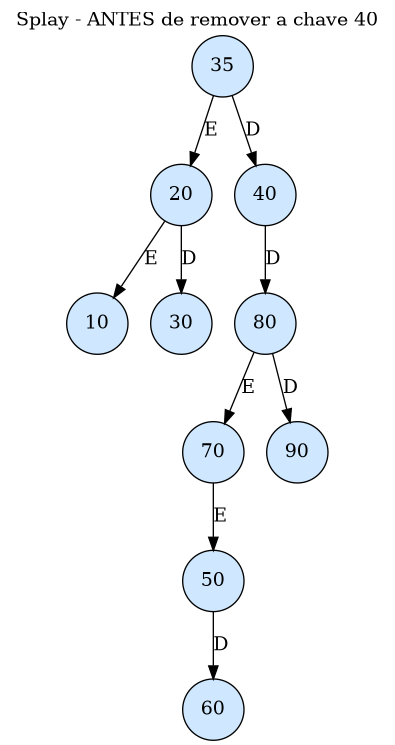
\includegraphics[width=0.75\linewidth]{figuras/splay_antes.png}\\[4pt]
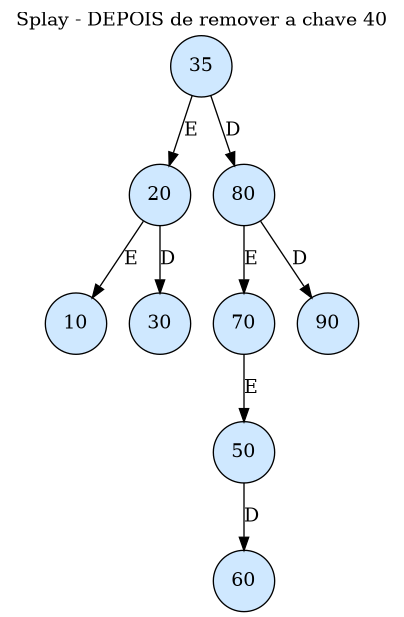
\includegraphics[width=0.75\linewidth]{figuras/splay_depois.png}
\caption{Árvore Splay antes e depois da remoção da chave 40. A remoção provoca um \textit{splay} do sucessor (chave 35) até a posição do nó removido, reorganizando toda a subárvore à direita de 20.}
\label{fig:splay}
\end{figure}

\begin{figure}[htbp]
\centering
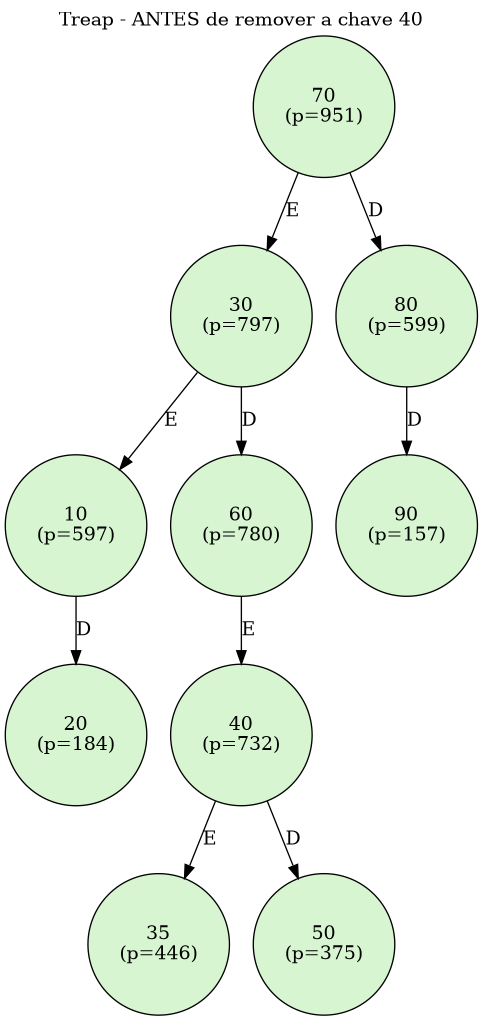
\includegraphics[width=0.55\linewidth]{figuras/treap_antes.png}\\[4pt]
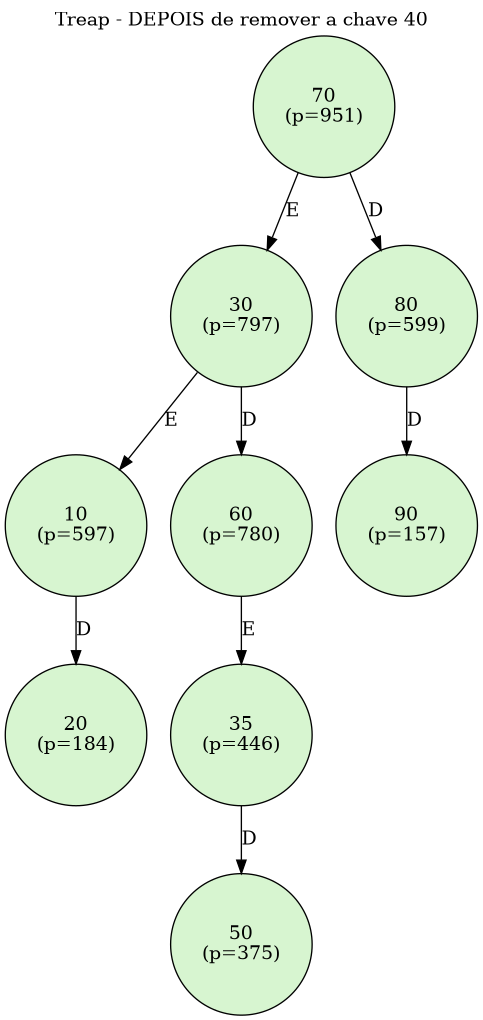
\includegraphics[width=0.55\linewidth]{figuras/treap_depois.png}
\caption{Árvore Treap antes e depois da remoção da chave 40, com a prioridade ($p$) de cada nó explícita. A remoção rotaciona o nó 40 para baixo em direção ao filho de maior prioridade até virar folha.}
\label{fig:treap}
\end{figure}

\begin{figure}[htbp]
\centering
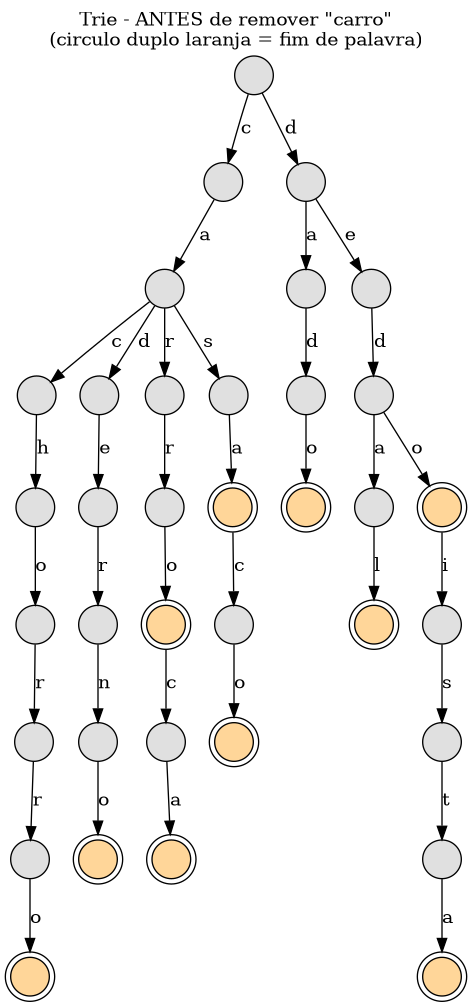
\includegraphics[width=0.75\linewidth]{figuras/trie_antes.png}
\caption{Trie construída a partir de 10 palavras com prefixos compartilhados. Cada aresta representa um único caractere; círculos duplos em laranja marcam nós de fim de palavra. Note o compartilhamento dos prefixos \textit{ca} e \textit{de}/\textit{da}.}
\label{fig:trie}
\end{figure}

\begin{figure}[htbp]
\centering
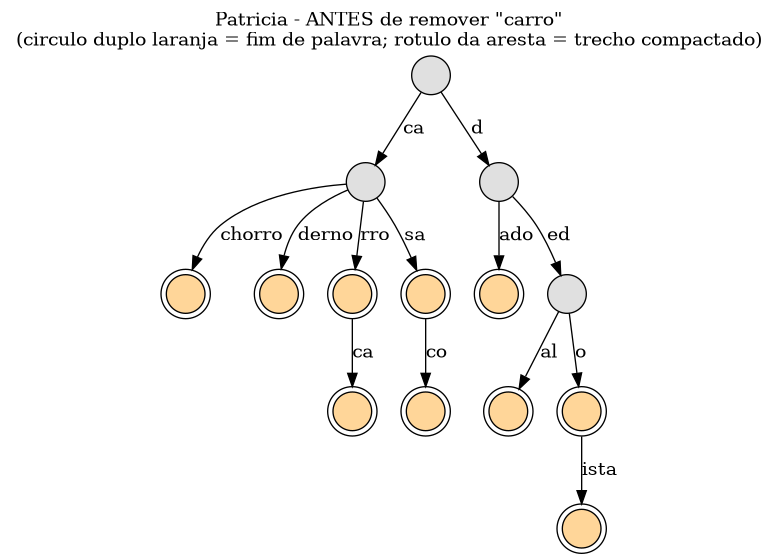
\includegraphics[width=0.85\linewidth]{figuras/patricia_antes.png}
\caption{Árvore Patricia para o mesmo conjunto de 10 palavras da Figura~\ref{fig:trie}. Arestas carregam subcadeias inteiras (ex.: \textit{chorro}, \textit{derno}, \textit{ista}), resultando em uma árvore consideravelmente mais rasa que a Trie equivalente.}
\label{fig:patricia}
\end{figure}

\begin{figure}[htbp]
\centering
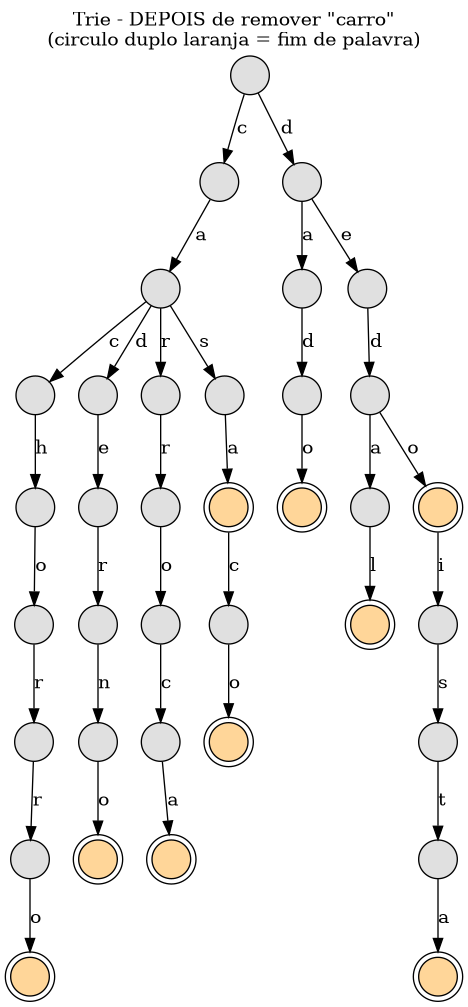
\includegraphics[width=0.75\linewidth]{figuras/trie_depois.png}\\[4pt]
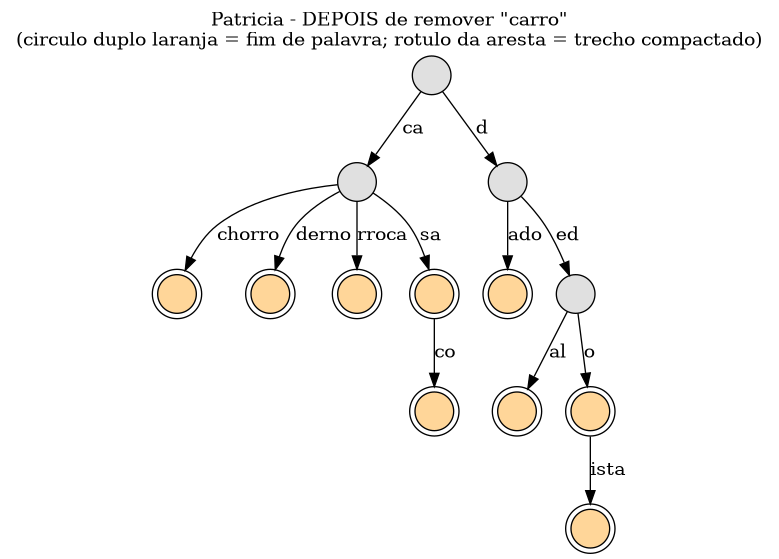
\includegraphics[width=0.85\linewidth]{figuras/patricia_depois.png}
\caption{Trie (acima) e Patricia (abaixo) após a remoção da palavra \textit{carro}. Em ambas, \textit{carroca} permanece intacta, pois apenas compartilhava o prefixo com \textit{carro} -- evidenciando que a remoção de uma chave não afeta chaves que apenas compartilham parte do caminho.}
\label{fig:trie-patricia-depois}
\end{figure}

\begin{figure}[htbp]
\centering
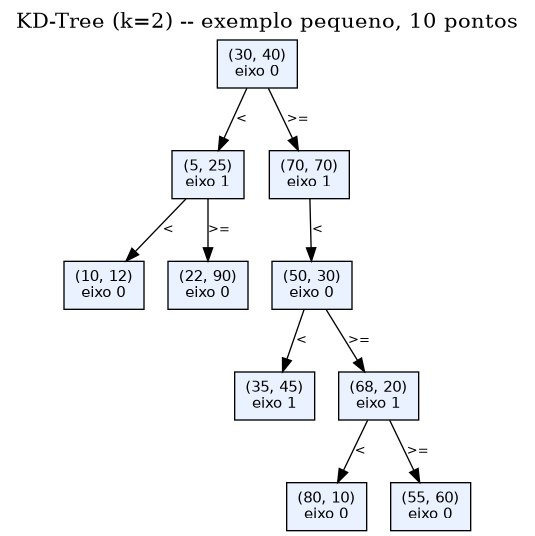
\includegraphics[width=0.75\linewidth]{figuras/kdtree_exemplo.png}
\caption{KD-Tree de exemplo com 10 pontos em $\mathbb{R}^2$. Cada nó indica a dimensão usada para particionar o espaço naquele nível (dimensão 0 = eixo $x$, dimensão 1 = eixo $y$), alternando ciclicamente com a profundidade.}
\label{fig:kdtree}
\end{figure}

A Figura~\ref{fig:trie-patricia-depois} ilustra bem o contraste central entre Trie e Patricia: a Trie precisa de um nó por caractere percorrido, enquanto a Patricia comprime caminhos sem ramificação em uma única aresta rotulada -- para o mesmo conjunto de 10 palavras, a Patricia (Figura~\ref{fig:patricia}) tem profundidade máxima 3, contra profundidade máxima 9 da Trie (Figura~\ref{fig:trie}).

% =====================================================================
\section{Análise de Complexidade e Comparação Teórica}

A Tabela~\ref{tab:complexidade} resume a complexidade assintótica das operações fundamentais de cada estrutura, incluindo BST e AVL como referência.

\begin{table}[htbp]
\centering
\caption{Complexidade assintótica das operações fundamentais}
\label{tab:complexidade}
\resizebox{\linewidth}{!}{%
\begin{tabular}{lccccc}
\toprule
\textbf{Estrutura} & \textbf{Busca} & \textbf{Inserção} & \textbf{Remoção} & \textbf{Construção} & \textbf{Espaço} \\
\midrule
BST (não balanceada) & $O(n)$ pior & $O(n)$ pior & $O(n)$ pior & $O(n\log n)$ & $O(n)$ \\
AVL & $O(\log n)$ & $O(\log n)$ & $O(\log n)$ & $O(n\log n)$ & $O(n)$ \\
Trie & $O(m)$ & $O(m)$ & $O(m)$ & $O(n\cdot m)$ & $O(n\cdot m\cdot|\Sigma|)$ \\
Patricia & $O(m)$ & $O(m)$ & $O(m)$ & $O(n\cdot m)$ & $O(n\cdot m)$ \\
Splay & $O(\log n)^{*}$ & $O(\log n)^{*}$ & $O(\log n)^{*}$ & $O(n\log n)$ & $O(n)$ \\
Treap & $O(\log n)^{\dagger}$ & $O(\log n)^{\dagger}$ & $O(\log n)^{\dagger}$ & $O(n\log n)$ & $O(n)$ \\
KD-Tree ($k$-D) & $O(\log n)^{\ddagger}$ & $O(\log n)^{\ddagger}$ & $O(n)$ & $O(n\log n)$ & $O(n)$ \\
\bottomrule
\multicolumn{6}{l}{\footnotesize $n$ = nº de chaves, $m$ = comprimento da chave, $|\Sigma|$ = tamanho do alfabeto.}\\
\multicolumn{6}{l}{\footnotesize $^{*}$amortizado; pior caso de uma única operação é $O(n)$.\quad$^{\dagger}$esperado (aleatoriedade das prioridades).}\\
\multicolumn{6}{l}{\footnotesize $^{\ddagger}$médio; degrada para $O(n)$ com dimensionalidade alta ou dados adversariais.}
\end{tabular}%
}
\end{table}

\textbf{Por que Trie e Patricia dependem de $m$, não de $n$:} em ambas, o custo de uma operação é proporcional ao número de símbolos percorridos até localizar ou inserir a chave, e não à quantidade de chaves já armazenadas -- por isso a busca não degrada com o crescimento de $n$, ao contrário de uma BST. A diferença entre as duas está no espaço: a Trie aloca um nó por símbolo mesmo em caminhos sem ramificação, enquanto a Patricia colapsa esses caminhos, tornando o número de nós internos proporcional a $n$ (uma chave a mais insere no máximo um nó interno novo), e não a $n \cdot m$.

\textbf{Por que Splay é amortizado, não pior-caso:} uma única sequência de acessos a elementos alternados nas extremidades da árvore pode gerar uma cadeia degenerada de profundidade $O(n)$ temporariamente; a garantia $O(\log n)$ só vale para o custo médio de uma sequência longa de operações, demonstrável pelo método do potencial. Isso contrasta com a AVL, que garante $O(\log n)$ mesmo numa única operação isolada, ao custo de manter um fator de balanceamento e rebalancear ativamente a cada modificação.

\textbf{Por que Treap é esperado, não garantido:} o balanceamento decorre inteiramente da aleatoriedade das prioridades sorteadas; com probabilidade $1/n!$ as prioridades podem ser sorteadas numa ordem que produz uma árvore degenerada (equivalente a inserir chaves já ordenadas numa BST comum sem rotações), mas essa probabilidade é desprezível na prática. A vantagem sobre a AVL é a simplicidade de implementação (a rotação decorre só da comparação de prioridade, sem manter altura ou fator de balanceamento).

\textbf{Por que a KD-Tree degrada com a dimensionalidade:} a poda por hiperplano na busca de vizinho mais próximo só é eficaz quando o volume podado a cada nível é uma fração significativa do espaço restante; à medida que $k$ cresce, a distância entre pontos tende a se homogeneizar (fenômeno conhecido como maldição da dimensionalidade) e a fração podada por nível diminui, aproximando o custo de uma varredura linear $O(n)$. A remoção é listada como $O(n)$ porque, ao contrário das demais operações, a implementação de referência não realiza um ajuste local: remover um nó interno exige reconstruir a subárvore correspondente para preservar o invariante de particionamento por eixo.

% =====================================================================
\section{Metodologia Experimental e Resultados}

\subsection{Metodologia}
Cada estrutura foi medida com \texttt{std::chrono::high\_resolution\_clock}, cronometrando blocos completos de operações (não operações isoladas, para reduzir ruído de medição). Splay, Treap e KD-Tree foram testados em cinco tamanhos de entrada ($N = 100$, $1\,000$, $10\,000$, $100\,000$ e, para a KD-Tree, também $200\,000$ pontos), gerados por um script determinístico (seed fixa) que reproduz os três padrões de dados originais: para a Splay, um bloco de inserção em ordem aleatória seguido de $5N$ acessos com 70\% concentrados em um subconjunto "quente" de 5\% das chaves (para evidenciar o efeito do \textit{splaying}); para a Treap, os cenários RANDOM, SORTED e REVERSE; para a KD-Tree, pontos uniformemente distribuídos e pontos concentrados em agrupamentos, em $[0,100]^2$. Trie e Patricia foram medidas com o conjunto de 1000 palavras fornecido, em inserção, busca e remoção de metade das palavras. Todas as medições foram gravadas em CSV (estrutura, bloco, operação, quantidade, tempo em ms), permitindo reconstrução e comparação posterior.

\subsection{Resultados}

A Figura~\ref{fig:grafico} mostra o tempo de inserção de Splay, Treap e KD-Tree em função de $N$, em escala log-log.

\begin{figure}[htbp]
\centering
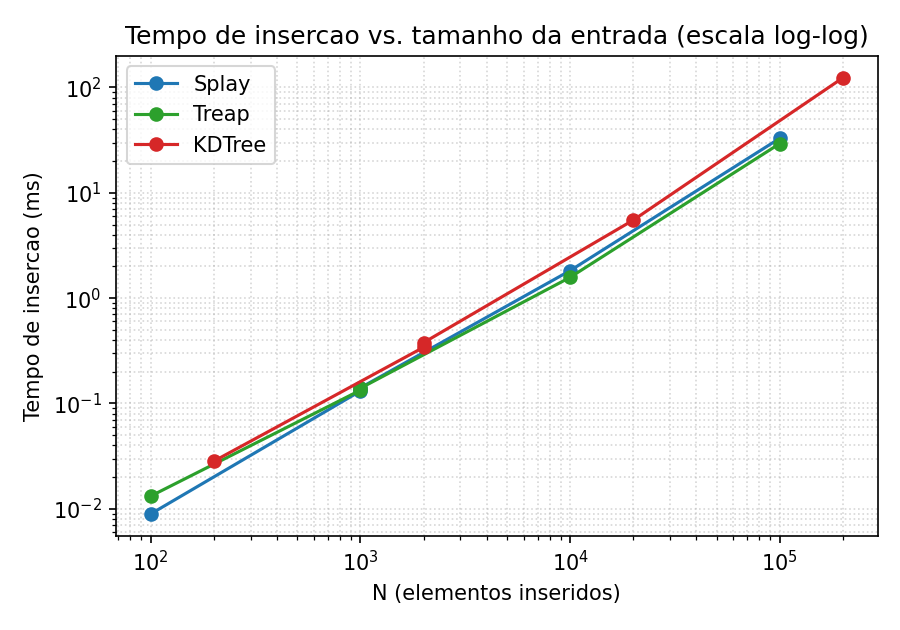
\includegraphics[width=\linewidth]{figuras/grafico_insercao.png}
\caption{Tempo de inserção vs. tamanho da entrada ($N$), escala log-log, para Splay (ordem aleatória), Treap (cenário RANDOM) e KD-Tree (pontos uniformes em 2D).}
\label{fig:grafico}
\end{figure}

A Tabela~\ref{tab:resultados} resume uma amostra dos tempos medidos para $N=1\,000$ (valor comum entre as cinco estruturas), permitindo comparação direta.

\begin{table}[htbp]
\centering
\caption{Tempo de execução para $N=1\,000$ (ou 1000 palavras, para Trie/Patricia)}
\label{tab:resultados}
\small
\resizebox{\linewidth}{!}{%
\begin{tabular}{lccc}
\toprule
\textbf{Estrutura} & \textbf{Inserção (ms)} & \textbf{Busca (ms)} & \textbf{Remoção (ms)} \\
\midrule
Splay      & 0,141 & 0,298\textsuperscript{a} & 0,004\textsuperscript{b} \\
Treap (RANDOM) & 0,134 & 0,036 & 0,067\textsuperscript{c} \\
Trie       & 0,249 & 0,012 & 0,056\textsuperscript{c} \\
Patricia   & 0,334 & 0,172 & 0,130\textsuperscript{c} \\
\bottomrule
\end{tabular}%
}

\vspace{2pt}
\footnotesize a: 5000 buscas (bloco ACCESS). \quad b: 50 remoções (bloco HOTSET). \quad c: remoção de metade das chaves/palavras (500).
\end{table}

\subsection{Discussão}
O gráfico log-log da Figura~\ref{fig:grafico} mostra as três curvas próximas de uma reta com inclinação levemente superior a 1, coerente com o comportamento teórico $O(n\log n)$ esperado para a construção de todas as três estruturas -- o crescimento super-linear observado (o tempo aumenta pouco mais que proporcionalmente a $N$) é justamente a assinatura do fator $\log n$. A KD-Tree consistentemente apresenta o maior tempo de inserção entre as três, mesmo em 2D; isso é coerente com o custo por nó ser maior (cada inserção compara vetores de coordenadas, não um único inteiro).

A busca na Trie (0,012~ms para 1000 buscas) é a mais rápida da tabela, consistente com sua complexidade $O(m)$ independente de $n$: para as palavras de tamanho moderado usadas no experimento, o custo por busca é pequeno e não cresce com o tamanho do dicionário. A Patricia, apesar de ter a mesma complexidade assintótica, apresentou busca mais lenta que a Trie no experimento; a causa provável é o custo constante mais alto por nó (comparação de subcadeias e uso de \texttt{std::map} para indexar filhos, em vez de acesso direto por índice de vetor como na Trie) -- um lembrete de que complexidade assintótica igual não implica desempenho prático igual.

A remoção na Splay (0,004~ms para 50 chaves do HOTSET) é discrepante em relação às demais remoções da tabela porque essas 50 chaves já haviam sido splayadas para perto da raiz pelo bloco ACCESS imediatamente anterior (por construção, o HOTSET é justamente o subconjunto mais acessado) -- um exemplo direto, e mensurável, do princípio de localidade temporal que fundamenta a árvore Splay.

% =====================================================================
\section{Aplicações, Análise Crítica e Discussão}

\subsection{Aplicações}
A \textbf{Trie} é a estrutura de escolha para autocompletar e correção ortográfica, onde a busca por prefixo em $O(m)$ permite listar sugestões instantaneamente conforme o usuário digita. A \textbf{Patricia} é preferível quando o volume de chaves é grande e a memória é escassa -- seu uso canônico é a busca por prefixo mais longo em tabelas de roteamento IP, onde milhões de prefixos precisam caber em memória de roteador. A \textbf{Splay} se destaca em sistemas de cache e estruturas com padrão de acesso desigual (poucos itens concentram a maioria dos acessos), como caches de tradução de páginas de memória. A \textbf{Treap} é atrativa quando se precisa de um conjunto ordenado com operações eficientes de \textit{split}/\textit{merge} e implementação simples, como em estruturas de dados persistentes e balanceamento de carga distribuído. A \textbf{KD-Tree} é a base de buscas por vizinho mais próximo em sistemas de informação geográfica, algoritmos de aprendizado de máquina baseados em vizinhança ($k$-NN) e detecção de colisão em computação gráfica.

\subsection{Vantagens e limitações observadas}
A principal vantagem prática da Treap, confirmada na implementação, é a simplicidade: o balanceamento inteiro decorre de uma comparação de prioridade, sem precisar manter ou recalcular altura/fator de balanceamento como na AVL. Em contrapartida, a Splay exigiu mais cuidado de implementação: os três casos de rotação (\textit{zig}, \textit{zig-zig}, \textit{zig-zag}) para cada lado (esquerda/direita) totalizam uma lógica consideravelmente mais longa e propensa a erros de ponteiro do que a Treap. Entre Trie e Patricia, a Patricia exigiu a lógica mais delicada de todo o trabalho: a divisão de uma aresta existente ao inserir uma chave que compartilha apenas um prefixo parcial com o rótulo daquela aresta precisa tratar corretamente os casos em que o prefixo comum é vazio, total ou parcial.

A generalização da KD-Tree para dimensão $k$ arbitrária (originalmente fixa em 2D) foi direta porque a lógica de alternância de eixo (\texttt{profundidade \% k}) já era escrita de forma genérica; a única mudança estrutural foi trocar coordenadas fixas (\texttt{double x, y}) por um vetor de tamanho variável.

\subsection{Teoria vs. experimento}
Os resultados experimentais da Seção~V foram, de forma geral, coerentes com a análise teórica da Seção~IV: o crescimento observado do tempo de inserção acompanhou o formato esperado de $O(n\log n)$ para as três estruturas testadas em múltiplos tamanhos. A principal divergência notada foi entre Trie e Patricia na operação de busca: a teoria prevê complexidade idêntica ($O(m)$ para ambas), mas o experimento mostrou a Patricia consistentemente mais lenta -- evidenciando que constantes ocultas pela notação assintótica (custo de comparação de subcadeias, indireção do \texttt{std::map}) podem dominar o tempo real para o tamanho de entrada testado.

\subsection{Possíveis extensões}
Entre as melhorias mais relevantes: (i) implementar reconstrução periódica ou rebalanceamento incremental na KD-Tree, hoje ausente, para evitar degradação após muitas remoções; (ii) substituir o \texttt{std::map<char,NoPatricia*>} por um vetor indexado, reduzindo a constante por nó da Patricia; (iii) estender os experimentos a distribuições adversariais (por exemplo, sequência de acessos adversarial contra a Splay) para observar o pior caso $O(n)$ isolado, hoje mascarado pela média amortizada.

% =====================================================================
\section{Conclusão}

As cinco estruturas estudadas resolvem, cada uma, uma limitação distinta das BSTs balanceadas clássicas. Trie e Patricia trocam a comparação de chaves atômicas por decomposição em símbolos, tornando o custo por operação proporcional ao comprimento da chave em vez do tamanho do conjunto -- a Patricia é estritamente mais econômica em espaço, à custa de uma implementação mais delicada. Splay e Treap alcançam balanceamento sem o custo de manutenção explícita da AVL, trocando garantia de pior caso por garantia amortizada (Splay) ou esperada (Treap); entre as duas, a Treap se mostrou a mais simples de implementar corretamente. A KD-Tree resolve um problema ortogonal às demais -- indexação multidimensional --, mas é a única cuja complexidade de busca degrada de forma mensurável com o crescimento da dimensionalidade.

Os experimentos confirmaram o comportamento assintótico esperado para inserção nas três estruturas testadas em escala (Splay, Treap, KD-Tree), com o gráfico log-log evidenciando o fator $\log n$ do custo teórico. A principal lição prática do trabalho é que complexidade assintótica idêntica (caso de Trie e Patricia na busca) não garante desempenho idêntico: a constante por operação, determinada por decisões de implementação como a estrutura de indexação de filhos, pode dominar o tempo observado para tamanhos de entrada realistas.

Quanto à escolha de estrutura para um problema específico: a Trie é preferível quando o alfabeto é pequeno e a velocidade de busca por prefixo é crítica; a Patricia, quando a memória é a restrição dominante; a Splay, quando o padrão de acesso é desigual e previsivelmente concentrado; a Treap, quando se deseja um conjunto ordenado balanceado com implementação simples; e a KD-Tree, sempre que a chave for inerentemente multidimensional e a dimensionalidade for baixa a moderada.

\begin{thebibliography}{99}

\bibitem{bentley1975}
BENTLEY, J. L. Multidimensional Binary Search Trees Used for Associative Searching. \textit{Communications of the ACM}, v.~18, n.~9, p.~509--517, 1975.

\bibitem{cormen2009}
CORMEN, T. H.; LEISERSON, C. E.; RIVEST, R. L.; STEIN, C. \textit{Introduction to Algorithms}. 3.~ed. Cambridge: MIT Press, 2009.

\bibitem{fredkin1960}
FREDKIN, E. Trie Memory. \textit{Communications of the ACM}, v.~3, n.~9, p.~490--499, 1960.

\bibitem{morrison1968}
MORRISON, D. R. PATRICIA --- Practical Algorithm To Retrieve Information Coded in Alphanumeric. \textit{Journal of the ACM}, v.~15, n.~4, p.~514--534, 1968.

\bibitem{sedgewick2011}
SEDGEWICK, R.; WAYNE, K. \textit{Algorithms}. 4.~ed. Boston: Addison-Wesley, 2011.

\bibitem{seidel1996}
SEIDEL, R.; ARAGON, C. R. Randomized Search Trees. \textit{Algorithmica}, v.~16, n.~4/5, p.~464--497, 1996.

\bibitem{sleator1985}
SLEATOR, D. D.; TARJAN, R. E. Self-Adjusting Binary Search Trees. \textit{Journal of the ACM}, v.~32, n.~3, p.~652--686, 1985.

\bibitem{vuillemin1980}
VUILLEMIN, J. A Unifying Look at Data Structures. \textit{Communications of the ACM}, v.~23, n.~4, p.~229--239, 1980.

\bibitem{github}
FARIA, G. A. \textit{Trabalho1 -- Estruturas em Árvores Avançadas}. GitHub, 2026. Disponível em: \url{https://github.com/SEU-USUARIO/SEU-REPOSITORIO}. Acesso em: 19 set. 2026.

\end{thebibliography}

\end{document}